This layer is the destination of all the instructions from the control layer go to. It contains the UR5's arm, its control box, and a polyscope for the UI.

\begin{figure}[h!]
	\centering
 	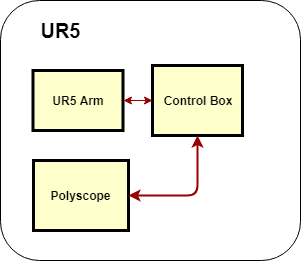
\includegraphics[width=0.60\textwidth]{images/UR5_Layer}
 \caption{UR5 layer diagram}
\end{figure}

\subsection{UR5 Arm}
This is the physical arm of the UR5. It receives instruction from the control box and act accordingly.

\subsubsection{Assumptions}
The arm is fully functional and can pick up at least 5 pounds.
It is connected to the control box.
It comes with the control box and polyscope.

\subsubsection{Responsibilities}
This arm takes in instruction from the UI. It moves accordingly to what the user instructions through the UI.


\subsubsection{Subsystem Interfaces}
The arm is connected to the control box as its interface.

\begin {table}[H]
\caption {UR5 Arm interfaces} 
\begin{center}
    \begin{tabular}{ | p{1cm} | p{6cm} | p{3cm} | p{3cm} |}
    \hline
    ID & Description & Inputs & Outputs \\ \hline
    \#xx & UR5 control box & \pbox{3cm}{Instructions(UR script)} & \pbox{3cm}{Position of arm}  \\ \hline
    \end{tabular}
\end{center}
\end{table}

\subsection{Control Box}
The control box is what allow the arm to receive instructions and move accordingly. It receives instruction from the UI through the polyscope or it can receive instructions from an outside source through a socket.

\subsubsection{Assumptions}
Functional and connects to the arm.
It comes with the arm and polyscope.

\subsubsection{Responsibilities}
The control box receive inputs and then outputs the instruction to the arm.

\subsubsection{Subsystem Interfaces}
The control box is connected to the arm and the polyscope. It is also controlling the connector that is on the wrist of the arm.

\begin {table}[H]
\caption {Control Box interfaces} 
\begin{center}
    \begin{tabular}{ | p{1cm} | p{6cm} | p{3cm} | p{3cm} |}
    \hline
    ID & Description & Inputs & Outputs \\ \hline
    \#xx & UR5 Arm & \pbox{3cm}{Position of Arm} & \pbox{3cm}{Waypoints \\ UR scripts}  \\ \hline
    \#xx & Polyscope & \pbox{3cm}{Instructions(UR script) \\ Waypoints \\ I/O control \\ Voltage} & \pbox{3cm}{Position of arm \\ I/O control\\ Voltage}  \\ \hline
    \#xx & Connector & \pbox{3cm}{N/A} & \pbox{3cm}{Voltage}  \\ \hline
    \end{tabular}
\end{center}
\end{table}

\subsection{Polyscope}
The polyscope is a UI that comes with the UR5. It is where all the script and control of the UR5 movements that can be instructed by writing a script.

\subsubsection{Assumptions}
The user is not using the polyscope as a way of sending the the instructions to the arm.
It is connected to the control box.
It comes with the control box and the arm.

\subsubsection{Responsibilities}
The emergency stop button is use to stop the arm immediately.

\subsubsection{Subsystem Interfaces}
The polyscope interface is the control box.

\begin {table}[H]
\caption {Polyscope interfaces} 
\begin{center}
    \begin{tabular}{ | p{1cm} | p{6cm} | p{3cm} | p{3cm} |}
    \hline
    ID & Description & Inputs & Outputs \\ \hline
    \#xx & UR5 control box & \pbox{3cm}{Position of arm \\ I/O control\\ Voltage} & \pbox{3cm}{Instructions(UR script) \\ Waypoints \\ I/O control \\ Voltage}  \\ \hline
    \end{tabular}
\end{center}
\end{table}

